%======================================================================
% University of Waterloo Thesis Template for LaTeX 
% Last Updated August 2023
% by IST Client Services, 
% University of Waterloo, 200 University Ave. W., Waterloo, Ontario, Canada
% FOR ASSISTANCE, please send mail to ist-helpdesk@uwaterloo.ca
%======================================================================
% Some important notes on using this template and making it your own...
% Modify "hyperref" package configuration below. 
% Search for: PDFTITLE, PDFSUBJECT, and PDFKEYWORDS.

% To create a PDF output that is optimized for double-sided printing: 
% 1) comment-out the \documentclass statement in the preamble below, and un-comment the second \documentclass line.
% 2) change the value assigned below to the boolean variable "PrintVersion" from " false" to "true".

%======================================================================
%   D O C U M E N T   P R E A M B L E

\documentclass[letterpaper,12pt,titlepage,oneside,final]{book}
% For PDF, suitable for double-sided printing, change the PrintVersion variable below to "true" and use this \documentclass line instead of the one above:
%\documentclass[letterpaper,12pt,titlepage,openright,twoside,final]{book}

% Some LaTeX commands I define for my own nomenclature.
% If you have to, it's easier to make changes to nomenclature once here than in a million places throughout your thesis!
\newcommand{\package}[1]{\textbf{#1}} % package names in bold text
\newcommand{\cmmd}[1]{\textbackslash\texttt{#1}} % command name in tt font 
\newcommand{\href}[1]{#1} % does nothing, but defines the command so the print-optimized version will ignore \href tags (redefined by hyperref pkg).
%\newcommand{\texorpdfstring}[2]{#1} % does nothing, but defines the command
% Anything defined here may be redefined by packages added below...

% This package allows if-then-else control structures.
\usepackage{ifthen}
\newboolean{PrintVersion}
\setboolean{PrintVersion}{false}

% Bibliography
\usepackage[
	style=numeric, % In-text citation style for APA, numeric otherwise
    giveninits=true,
]{biblatex}
\addbibresource{uw-ethesis.bib}

%\usepackage{nomencl} % For a nomenclature (optional; available from ctan.org)
\usepackage{amsmath,amssymb,amstext} % Lots of math symbols and environments
\usepackage[pdftex]{graphicx} % For including graphics N.B. pdftex graphics driver 

%---------------------------------------------
%	TABLES
%---------------------------------------------

\usepackage{booktabs} % Required for better horizontal rules in tables

\usepackage{array} % Required for manipulating table columns

\newcolumntype{R}[1]{>{\raggedleft\arraybackslash}p{#1}} % Define a new right-aligned paragraph column type
\newcolumntype{L}[1]{>{\raggedright\arraybackslash}p{#1}} % Define a new left-aligned (no justification) paragraph column type
\newcolumntype{C}[1]{>{\centering\arraybackslash}p{#1}} % Define a new centered paragraph column type

% Hyperlinks make it very easy to navigate an electronic document.
% In addition, this is where you should specify the thesis title and author as they appear in the properties of the PDF document.
% Use the "hyperref" package 
% N.B. HYPERREF MUST BE THE LAST PACKAGE LOADED; ADD ADDITIONAL PKGS ABOVE
\usepackage[pdftex,pagebackref=false]{hyperref} % with basic options
%\usepackage[pdftex,pagebackref=true]{hyperref}
		% N.B. pagebackref=true provides links back from the References to the body text. This can cause trouble for printing.
\hypersetup{
    plainpages=false,       % needed if Roman numbers in frontpages
    unicode=false,          % non-Latin characters in Acrobat’s bookmarks
    pdftoolbar=true,        % show Acrobat’s toolbar?
    pdfmenubar=true,        % show Acrobat’s menu?
    pdffitwindow=false,     % window fit to page when opened
    pdfstartview={FitH},    % fits the width of the page to the window
    pdftitle={Explaining embedding results for scoring alignments},
    pdfauthor={Riley Gavigan},
    pdfsubject={Deep Learning},
    pdfkeywords={deep learning} {machine learning} {bioinformatics},       % list of keywords
    pdfnewwindow=true,      % links in new window
    colorlinks=true,        % false: boxed links; true: colored links
    linkcolor=blue,         % color of internal links
    citecolor=green,        % color of links to bibliography
    filecolor=magenta,      % color of file links
    urlcolor=cyan           % color of external links
}
\ifthenelse{\boolean{PrintVersion}}{   % for improved print quality, change some hyperref options
\hypersetup{	% override some previously defined hyperref options
%    colorlinks,%
    citecolor=black,%
    filecolor=black,%
    linkcolor=black,%
    urlcolor=black}
}{} % end of ifthenelse (no else)

\usepackage[automake,toc,abbreviations]{glossaries-extra} % Exception to the rule of hyperref being the last add-on package
% If glossaries-extra is not in your LaTeX distribution, get it from CTAN (http://ctan.org/pkg/glossaries-extra), 
% although it's supposed to be in both the TeX Live and MikTeX distributions. There are also documentation and 
% installation instructions there.

% Setting up the page margins...
% uWaterloo thesis requirements specify a minimum of 1 inch (72pt) margin at the
% top, bottom, and outside page edges and a 1.125 in. (81pt) gutter margin (on binding side). 
% While this is not an issue for electronic viewing, a PDF may be printed, and so we have the same page layout for both printed and electronic versions, we leave the gutter margin in.
% Set margins to minimum permitted by uWaterloo thesis regulations:
\setlength{\marginparwidth}{0pt} % width of margin notes
% N.B. If margin notes are used, you must adjust \textwidth, \marginparwidth
% and \marginparsep so that the space left between the margin notes and page
% edge is less than 15 mm (0.6 in.)
\setlength{\marginparsep}{0pt} % width of space between body text and margin notes
\setlength{\evensidemargin}{0.125in} % Adds 1/8 in. to binding side of all 
% even-numbered pages when the "twoside" printing option is selected
\setlength{\oddsidemargin}{0.125in} % Adds 1/8 in. to the left of all pages when "oneside" printing is selected, and to the left of all odd-numbered pages when "twoside" printing is selected
\setlength{\textwidth}{6.375in} % assuming US letter paper (8.5 in. x 11 in.) and side margins as above
\raggedbottom

% The following statement specifies the amount of space between paragraphs. Other reasonable specifications are \bigskipamount and \smallskipamount.
\setlength{\parskip}{\medskipamount}

% The following statement controls the line spacing.  
% The default spacing corresponds to good typographic conventions and only slight changes (e.g., perhaps "1.2"), if any, should be made.
\renewcommand{\baselinestretch}{1} % this is the default line space setting

% By default, each chapter will start on a recto (right-hand side) page.
% We also force each section of the front pages to start on a recto page by inserting \cleardoublepage commands.
% In many cases, this will require that the verso (left-hand) page be blank, and while it should be counted, a page number should not be printed.
% The following statements ensure a page number is not printed on an otherwise blank verso page.
\let\origdoublepage\cleardoublepage
\newcommand{\clearemptydoublepage}{%
  \clearpage{\pagestyle{empty}\origdoublepage}}
\let\cleardoublepage\clearemptydoublepage

% Define Glossary terms (This is properly done here, in the preamble and could also be \input{} from a separate file...)
% Main glossary entries -- definitions of relevant terminology
\pagestyle{fancy}
\fancyhf{}
\renewcommand{\headrulewidth}{0pt}
\fancyhead[R]{\small\textit{Gavigan, Riley}}
\fancyhead[L]{\small\textbf{Page \thepage{} of \pageref*{LastPage}}}

\newglossaryentry{transformer}
{
name=transformer,
description={a type of neural network architecture used to solve the problem of transduction or transformation of input sequences into output sequences in deep learning applications using self-attention}
}

\newglossaryentry{amino acids}
{
name=amino acid,
description={molecules that combine to form proteins, containing both an amino and a carboxyl group}
}

\newglossaryentry{peptide}
{
name=peptide,
description={a compound consisting of two or more amino acids linked in a chain, the carboxyl group of each acid being joined to the amino group of the next},
plural={peptides}
}

\newglossaryentry{residue}
{
name=residue,
description={a single unit that makes up a polymer, such as an amino acid in a polypeptide chain},
plural={residues}
}

% List of Abbreviations
\newabbreviation{NLP}{NLP}{Natural Language Processing}
\newabbreviation{BLAST}{BLAST}{Basic Local Alignment Search Tool}
\newabbreviation{BERT}{BERT}{Bidirectional Encoder Representations from Transformers}
\newabbreviation{ALBERT}{ALBERT}{A Lite BERT}
\newabbreviation{RoBERTa}{RoBERTa}{Robustly Optimized BERT}
\newabbreviation{T5}{T5}{Text-To-Text Transfer Transformer}
\newabbreviation{ENNA}{ENNA}{Evolutionary Neural Network Algorithm}
\newabbreviation{MSA}{MSA}{Multiple Sequence Alignments}
\newabbreviation{LLM}{LLM}{Large Language Models}
\newabbreviation{LoRA}{LoRA}{Low-Rank Adaptation}
\newabbreviation{CDD}{CDD}{Conserved Domain Database}
\newabbreviation{BLOSUM}{BLOSUM}{BLOcks SUbstitution Matrix}
\makeglossaries

%======================================================================
%   L O G I C A L    D O C U M E N T
% The logical document contains the main content of your thesis.
% Being a large document, it is a good idea to divide your thesis into several files, each one containing one chapter or other significant chunk of content, so you can easily shuffle things around later if desired.
%======================================================================
\begin{document}

%----------------------------------------------------------------------
% FRONT MATERIAL
% title page, examining committee membership (for PhD Thesis only), declaration, borrowers' page, abstract, acknowledgements,
% dedication, table of contents, list of tables, list of figures, nomenclature, etc.
%----------------------------------------------------------------------
% T I T L E   P A G E
\begin{titlepage}
        \begin{center}
        \vspace*{1.0cm}

        \Huge
        {\bf Explaining embedding results for scoring alignments }

        \large
        Final Progress Report \\

        \vspace*{1.0cm}

        \normalsize
        by \\

        \vspace*{1.0cm}

        \Large
        Riley Gavigan \\

        \vspace*{3.0cm}

        \normalsize
        CS 4490Z \\
        Thesis Supervisor: Lucian Ilie \\ 
        Course Instructor: Nazim Madhavi \\

        \vspace*{2.0cm}

        Department of Computer Science \\
        University of Western Ontario, London, N6A 5B7, Ontario, Canada \\
        \today \\

        \vspace*{1.0cm}
        \end{center}
\end{titlepage}

% Define a new chapter format that doesn't display the chapter number
\titleformat{\chapter}[display]
  {\normalfont\huge\bfseries}{}{0pt}{\Huge}

\setcounter{page}{2}

\cleardoublepage
\phantomsection

\printglossary

% L I S T   O F   A B B R E V I A T I O N S
\renewcommand*{\abbreviationsname}{Abbreviations}
\printglossary[type=abbreviations]
\cleardoublepage
\phantomsection

% A B S T R A C T
% ---------------
\chapter*{Structured Abstract}
\addcontentsline{toc}{chapter}{Structured Abstract}

\subsubsection*{Context and motivation}
The \textit{E}-score protein alignment scoring method \autocite{Ashrafzadeh:2023} outperforms state-of-the-art methods, supported by comparing ProtT5 \autocite{Elnaggar:2021} \textit{E}-score results with BLOSUM45 \autocite{Henikoff:1992}.

This research aimed to understand \textit{E}-score results, building upon the observation that mean cosine similarity results between two embeddings are not evenly distributed.

By understanding the underlying causes of the observed results, we can improve the \textit{E}-score method. Insights can be used to fine-tune the transformer models \autocite{Elnaggar:2021, Rives:2021} and performance of embeddings.

\subsubsection*{Research questions}
\begin{itemize}
    \item{What properties of embeddings produce better cosine similarity results?}
    \item{Why do cosine similarity results primarily fall within a positive range?}
    \item{How can models be fine-tuned to produce better embeddings?}
\end{itemize}

\subsubsection*{Principal ideas}
Positive cosine similarity results imply the produced embeddings are mostly similar. Comparing different embedding types provides insight into their distributions. Through these comparisons, conclusions about properties that improve \textit{E}-score results were drawn.

\subsubsection*{Research methodology}
This research is a data science investigation to obtain insight about the embeddings and cosine similarity results in the \textit{E}-score method.

\subsubsection*{Anticipated results}
This study primarily aimed to obtain insight and knowledge for the \textit{E}-score method, specifically:
\begin{itemize}
    \item{Knowledge about the distributions of different embedding types}
    \item{Knowledge about the cosine similarity between embeddings}
    \item{Insight to fine-tune and improve models}
\end{itemize}

\subsubsection*{Novelty}
By building upon a novel method for scoring protein alignments using cosine similarity \autocite{Ashrafzadeh:2023}, novel conclusions about embeddings and cosine similarity were made, leading to further research that can improve embeddings and models.

\subsubsection*{Impact}
Improvements in transformer models for the \textit{E}-score alignment scoring method can be made through the insight this research found. Improvements may also be applicable to \gls{NLP} Models such as T5 \autocite{Raffel:2020}.

\subsubsection*{Progress and completed work}
Insight into properties behind embedding type distributions was obtained. From these properties, cosine similarity results were explained. These properties were explained through conducted research and simulation in combination with insight from biochemical background research.

\subsubsection*{Limitations}
No limitations are known to exist in this research.

\cleardoublepage
\phantomsection

% T A B L E   O F   C O N T E N T S
% ---------------------------------
\renewcommand\contentsname{Table of Contents}
\tableofcontents
\cleardoublepage
\phantomsection

% L I S T   O F   S Y M B O L S
% ---------------------------
\cleardoublepage
\phantomsection

% Change page numbering back to Arabic numerals
\pagenumbering{arabic}
 

%----------------------------------------------------------------------
% MAIN BODY
% We suggest using a separate file for each chapter of your thesis.
% Start each chapter file with the \chapter command.
% Only use \documentclass or \begin{document} and \end{document} commands in this master document.
% Tip: Putting each sentence on a new line is a way to simplify later editing.
%----------------------------------------------------------------------
%======================================================================
\chapter{Introduction}
%======================================================================

Proteins are one of the four molecules of life. Finding similarities among protein sequences is essential in identifying protein structure and function. This is done by computing alignments between sequences.

The \textit{E}-score method is a method to compute alignments between sequences using contextual embeddings produced by \gls{transformer} models \cite{Ashrafzadeh:2023}. This method uses several different transformer models based off of models in \gls{NLP}.

This research addresses the results observed for the \textit{E}-score method. Namely, I explain the observed cosine similarity results and explain significant differences and similarities between the models used (Table \ref{tab:transformers}), both qualitative and quantitative. Combining the comparison of models with visualization and analysis of embedding vector and cosine similarity distributions, I propose the contributing factors to better \textit{E}-score performance.

Using inference about the proposed factors contributing to \textit{E}-score performance, I describe the procedure and techniques for fine-tuning ProtT5 and other models to produce better embeddings for sequence alignment.

\section{Thesis outline}
Chapter 2 provides a reader with background on important concepts and details discussed later in the thesis. Chapter 3 outlines the materials and methods used in the research conducted on the \textit{E}-score method. Chapter 4 provides the results from analysis performed in the data science investigation. Chapter 5 concludes the study by addressing the research questions outlined in the thesis proposal, and discusses impact and novelty of the results.
%======================================================================
\chapter{Background}
%======================================================================
\section{Natural Language Processing}
Natural Language Processing is the branch of artificial intelligence that deals with providing computers with the ability to understand text and spoken words, similar to how human being do \cite{Khurana:2023}. \gls{NLP} includes tasks such as summarization, sentiment analysis, and spam detection \cite{Khurana:2023}.

One significant advancement within \gls{NLP} was the introduction of \gls{transformer} models \cite{Vaswani:2017}. Before the introduction of Transformers within NLP, neural networks such as word2vec \cite{Mikolov:2013} and GloVe \cite{Pennington:2014} generated contextual independent embedding vectors for words. Transformer models such as T5, BERT, ALBERT, RoBERTa, and XLNet outperformed these models with the introduction of contextual embeddings generated through self-attention \cite{Vaswani:2017}.

The \gls{transformer} models used in \gls{NLP} vary significantly. Examples of differences between models includes with architecture, training procedure, and size. These differences contribute to different use cases and performance between models. The models used in the \textit{E}-score method for protein sequence alignment are based on the models introduced below for NLP. Comparison between the GLUE benchmark scores for these models is shown in Table \ref{tab:glue}

\subsection{T5}
\gls{T5} uses a text-to-text approach using the \gls{transformer} architecture. That is, T5's input and output are always text strings \cite{Raffel:2020}. It uses both the encoder and decoder from the transformer architecture, and relies on \gls{transfer learning} to fine-tune the model on downstream tasks. An example of T5's input and output is shown in Figure \ref{fig:t5example}.

\begin{figure}
    \begin{center}
	   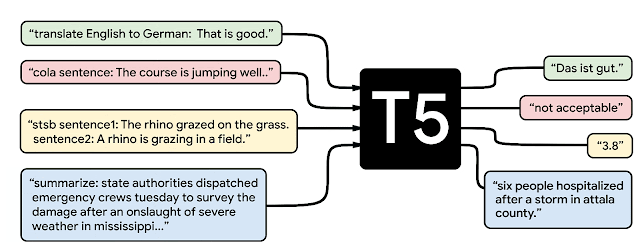
\includegraphics[width=0.75\linewidth]{figures/t5example.png}
    \end{center}
    \caption{Diagram of T5's text-to-text framework. Each task uses text as the model input, which is trained to generate some target text \cite{Raffel:2020}.}
    \label{fig:t5example}
\end{figure}

By training \gls{T5} with fill-in-the-blank-style \gls{denoising} objectives, where T5 was trained to recover missing words in the input, and using transfer learning on smaller labeled datasets, T5 was able to achieve state-of-the-art \gls{NLP} performance \cite{Raffel:2020}.

\subsection{BERT, ALBERT, and RoBERTa}
\gls{BERT} achieved state-of-the-art \gls{NLP} performance at the time of it being published \cite{Devlin:2018}. ALBERT and RoBERTa are both derivations of BERT, and \gls{T5} also drew significant inspiration from BERT, such as the \gls{denoising} objective being inspired by BERT's masked language modeling objective.

\gls{BERT} is an encoder-only model that applies bidirectional training using the "masked language modeling" objective that was created for the model. This contrasts the previous framework where models read the text input sequentially, allowing for a deeper sense of context. Masked Language Modeling works by replacing 15\% of the words in an input sequence being replaced with a "MASK" token, which the model attempts to predict the original value of based on the context from the other words \cite{Devlin:2018}.

\gls{ALBERT} addresses the limitations of training time and GPU/TPU memory by presenting parameter-reduction techniques for \gls{BERT} \cite{Zhenzhong:2020}.

\gls{RoBERTa} addresses the observation that \gls{BERT} was significantly under-trained. RoBERTa improved upon BERT by training longer, removing the next-sentence pretraining objective from BERT, and training with larger mini-batches and learning rates \cite{Liu:2019}.

\subsection{XLNet}
XLNet is a model that overcomes the pretrain-finetune discrepency that \gls{BERT} suffers from because it relies on masking the input during training \cite{Yang:2022}. XLNet is a decoder-only model (also known as autoregressive) that overcomes BERT's limitations because of it's autoregressive formulation.

XLNet outperforms \gls{BERT} significantly on 20 tasks, such as question answering and sentiment analysis \cite{Yang:2022}.

\begin{table*} % Two column table
	\caption{GLUE benchmark scores \cite{Wang:2019} for the Natural Language Processing models that serve as foundation for the \textit{E}-score models.}
	\centering
    \vspace{1mm}
	\begin{tabular}{ |c|c|c|c|c|c|c|c|c|c|c| }
		\toprule
		Model & Avg & CoLA & SST-2 & MRPC & STS-B & QQP & MNLI & RTE & WNLI\\
		\midrule
		T5 & 88.7 & 71.6 & 97.5 & 92.8 & 93.1 & 75.1 & 92.1 & 92.8 & 94.5 \\
        XLNet & 87.5 & 70.2 & 97.1 & 92.9 & 93.0 & 74.7 & 90.9 & 88.5 & 92.5\\
		ALBERT & 87.3 & 69.1 & 97.1 & 93.4 & 92.5 & 74.2 & 91.1 & 89.2 & 91.8\\
        RoBERTa & 86.4 & 67.8 & 96.7 & 92.3 & 92.2 & 74.3 & 90.5 & 88.2 & 89.0 \\
		\bottomrule
	\end{tabular}
	\label{tab:glue}
\end{table*}

\section{Sequence alignment}
Sequence similarity is essential in sequence analysis within bioinformatics \cite{Ofer:2021}. Peptide sequence alignment is the most complex case, with a language of 20 common \gls{amino acids} forming a theoretically countably infinite amount of unique \gls{peptide} sequences shown in Equation \ref{eq:peptideinfinity} by taking the n-ary Cartesian product.

\begin{equation}
    {Theoretical\, Limit} = \prod_{k=1}^{\infty} |A| = \prod_{k=1}^{\infty} 20 = 20 \times 20 \times \ldots
    \label{eq:peptideinfinity}
\end{equation}

While there is theoretically a countably infinite number of \gls{peptide} sequences, the observed sequences in living organisms are constrained by biological, genetic, and functional factors. For example, the average eukaryotic protein size is \(353 \pm 62.5\) \glspl{residue} \cite{Nevers:2023}. 

Databases such as UniProt \cite{UniProt:2023} and PeptideAtlas \cite{PeptideAtlas:2006} are repositories filled with \gls{peptide} sequences. UniProt contains over 250 million unique peptide sequences and counting, showcased in Figure \ref{fig:uniprot}.

\begin{figure}
    \begin{center}
	   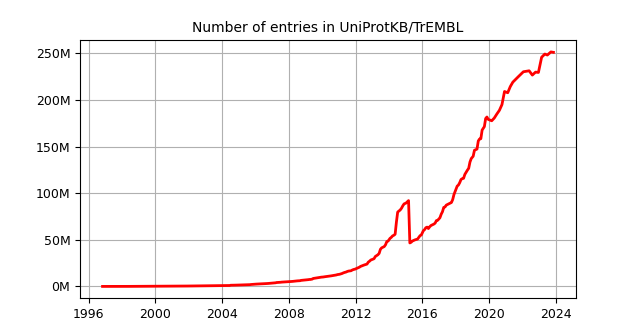
\includegraphics[width=0.75\linewidth]{figures/uniprot.png}
    \end{center}
    \caption{UniProtKB protein database release statistics as of May 2023 \cite{UniProt:2023}.}
    \label{fig:uniprot}
\end{figure}

Peptide sequences are not completely random because of the constraints imposed on them. Similar to letters or words in a given language within natural language, the frequency of each amino acid observed in nature is not equally distributed \cite{Beals:1999}, which can be observed in Figure \ref{fig:aafreq}.

\begin{figure}
    \begin{center}
	   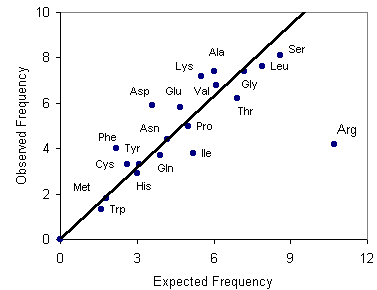
\includegraphics[width=0.5\linewidth]{figures/aafreq.png}
    \end{center}
    \caption{Observed frequency versus expected frequency of the 20 amino acids in vertebrates \cite{Beals:1999}}
    \label{fig:aafreq}
\end{figure}

Proteins are also not completely random and form different secondary structures as part of the tertiary and quaternary structure of a protein. The most common of these secondary structures are \(\alpha\) helices and \(\beta\) pleated sheets \cite{Ma:2018}. Because of the nature of proteins, algorithms such as an \gls{ENNA} are able to distinguish natural proteins from randomly generated proteins with an accuracy of over 94\% \cite{Lucrezia:2012}.

Finding similarities among protein sequences is essential in identifying protein structure and function. This is done by computing alignments between sequences. The \gls{BLAST} program\footnote{Exceeds 108,000 citations, according to Google Scholar.} is one of the most widely used tools in science \cite{Atschul:1990}. An essential part of BLAST is the scoring function; the most widely used functions are provided by the BLOSUM matrices \cite{Henikoff:1992}.

The \textit{E}-score protein alignment scoring method \cite{Ashrafzadeh:2023} is another one of these scoring functions, and outperforms state-of-the-art methods. The improved performance was supported by comparing ProtT5 \cite{Elnaggar:2021} \textit{E}-score results with BLOSUM45 \cite{Henikoff:1992,Ashrafzadeh:2023}.

\section{\textit{E}-score}
\textit{E}-score uses \gls{transformer} models to produce contextual embeddings for the \glspl{residue} in \gls{peptide} sequences. Model information is available in Table \ref{tab:transformers}. These models are based off of their \gls{NLP} equivalents \cite{Raffel:2020, Devlin:2018, Zhenzhong:2020, Yang:2022, Rives:2021}.

Contextual embeddings are embeddings produced by the self-attention mechanism in the \gls{transformer} architecture \cite{Vaswani:2017}. Similar to word embeddings in \gls{NLP}, they describe the position of a \gls{residue} in a high-dimensional vector space. Contextual embeddings have many important applications in biology, including structure prediction \cite{Senior:2020, Yang:2019, Jumper:2021} and function prediction \cite{Kulmanov:2019, Gligorijevic:2021, Lai:2021}. 

\begin{table*} % Two column table
	\caption{Transformer models available in the \textit{E}-score method; \(n=\) number of residues. ProtT5, ProtBert, ProtAlbert, and ProtXLNet come from ProtTrans \cite{Elnaggar:2021}. ESM1b and ESM2 come from the Meta Fundamental AI Research Protein Team \cite{Rives:2021}.}
	\centering
	\begin{tabular}{ |c|c|c|c|c| }
		\toprule
		Model & Architecture & Embedding Dim & Pre-Trained Dataset \\
		\midrule
		ProtT5 & Encoder-Decoder & n * 1024 & UniRef50 \\
        ESM1b & Encoder & n * 1280 & UniRef50 \\
        ESM2 & Encoder & n * 1280 & UniRef50 \\
		ProtBert & Encoder & n * 1024 & UniRef100 \\
		ProtAlbert & Encoder & n * 4096 & UniRef100 \\
        ProtXLNet & Decoder & n * 1024 & UniRef100 \\
		\bottomrule
	\end{tabular}
	\label{tab:transformers}
\end{table*}

The \textit{E}-score alignment method is another application for these embeddings, outperforming the state-of-the-art methods \cite{Ashrafzadeh:2023} by completely changing the way alignments are computed.

The embedding vector produced for each protein \gls{residue} varies based on the model that was used. For example, the embedding for a protein sequence of 310 residues using ProtT5 will have the dimensions [310, 1024]. The embedding dimensions are outlined in Table \ref{tab:transformers}. The dimensionality of the embedding vectors represents the number of features encoded in the embedding, and is a fixed value for a given model.

\subsection{Calculations}
The embeddings produced by a model for a protein \(P\), calculated in Equation \ref{eq:embedding}, are used as the input to calculate the cosine similarity.

\begin{equation}
    E(P) = GetEmbeddings(Model = ProtT5)
    \label{eq:embedding}
\end{equation}

Calculating the cosine similarity between two vectors \(A = (A_i)_{i=1..n}\) and \(B = (B_i)_{i=1..n}\) is shown in Equation \ref{eq:cossim}.

\begin{equation}
    \begin{aligned}
        CosSim(A, B) = cos(\theta) \equiv \frac{A \cdot B}{\Vert A \Vert \Vert B \Vert} %\\ 
        \equiv \frac{\sum\limits_{i=1}^{n} A_iB_i}{\sqrt{\sum\limits_{i=1}^{n} A_i^2}\sqrt{\sum\limits_{i=1}^{n} B_i^2}}
    \end{aligned}
	\label{eq:cossim}
\end{equation}

\textit{E}-score is calculated by taking the cosine similarity between the embedding vector for two \glspl{residue} (\(i, j\)), shown in Equation \ref{eq:escore} where \(P_1\) and \(P_2\) are proteins \cite{Ashrafzadeh:2023}.

\begin{equation}
    \textit{E}\mbox{-}score(i,j) = CosSim(E(P_1)_i, E(P_2)_j)
    \label{eq:escore}
\end{equation}

In calculating sequence alignment using the \textit{E}-score method, the cosine similarity results were mostly  mostly less than \(\frac{\pi}{2}\). It was also determined that ProtT5 performed better than the other models \cite{Ashrafzadeh:2023}.

Below are two examples that demonstrate obtaining the \textit{E}-score between two protein sequences. 
\begin{enumerate}
    \item{Two protein sequences, \(P_1\) and \(Q_1\), are highly similar and have diverged slightly through evolution. The embedding vectors produced by any of the Transformer models within \textit{E}-score for these sequences should be highly similar. Calculating the cosine similarity between the embedding vectors produced for \(P_1\) and \(Q_2\) should produce a result that is close to \(1\). The alignment score produced by the \textit{E}-score method through dynamic programming should be high.}
    \item{Two protein sequences, \(P_2\) and \(Q_2\), are very different and have diverged extensively through evolution. The embedding vectors produced for these sequence should be highly dissimilar. Calculating the cosine similarity between the embedding vectors produced for \(P_2\) and \(Q_2\) should produce a result that is close to \(-1\). The alignment score produced by the \textit{E}-score method through dynamic programming should be low.}
\end{enumerate}

\subsection{Transformers}
The \gls{transformer} models used in the \textit{E}-score method described in Table \ref{tab:transformers} vary in performance.

\begin{figure} % Single column figure
    \begin{center}
	   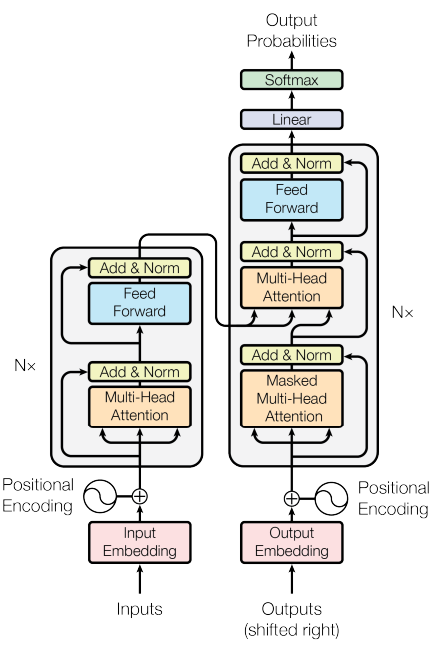
\includegraphics[width=0.6\linewidth]{figures/transformer.png}
    \end{center}
	\caption{Transformer model architecture \cite{Vaswani:2017}. Encoder is on the left; decoder is on the right.}
    \vspace{-5mm}
	\label{fig:transformer}
\end{figure}

\if{false}
\section{Fine-tuning}
\fi
%%======================================================================
\chapter{Materials \& Methods}
%======================================================================
%%======================================================================
\chapter{Results}
%======================================================================
%%======================================================================
\chapter{Conclusion}
%======================================================================

%----------------------------------------------------------------------
% END MATERIAL
% Bibliography, Appendices, Index, etc.
%----------------------------------------------------------------------

% Bibliography

% The following statement selects the style to use for references.  
% It controls the sort order of the entries in the bibliography and also the formatting for the in-text labels.
% This specifies the location of the file containing the bibliographic information.  
% It assumes you're using BibTeX to manage your references (if not, why not?).
\cleardoublepage % This is needed if the "book" document class is used, to place the anchor in the correct page, because the bibliography will start on its own page.
% Use \clearpage instead if the document class uses the "oneside" argument
\phantomsection  % With hyperref package, enables hyperlinking from the table of contents to bibliography             
% The following statement causes the title "References" to be used for the bibliography section:
\renewcommand*{\bibname}{References}

% Add the References to the Table of Contents
\addcontentsline{toc}{chapter}{\textbf{References}}

\printbibliography
% Tip: You can create multiple .bib files to organize your references. 
% Just list them all in the \bibliogaphy command, separated by commas (no spaces).

% The following statement causes the specified references to be added to the bibliography even if they were not cited in the text. 
% The asterisk is a wildcard that causes all entries in the bibliographic database to be included (optional).
\nocite{*}
%----------------------------------------------------------------------

% Appendices

% The \appendix statement indicates the beginning of the appendices.
%\appendix
% Add an un-numbered title page before the appendices and a line in the Table of Contents
%\chapter*{APPENDICES}
%\addcontentsline{toc}{chapter}{APPENDICES}
% Appendices are just more chapters, with different labeling (letters instead of numbers).
%\chapter[PDF Plots From Matlab]{Matlab Code for Making a PDF Plot}
\label{AppendixA}
% Tip 4: Example (above) of how to get a shorter chapter title for the Table of Contents 
%======================================================================
\section{Using the Graphical User Interface}
Properties of Matab plots can be adjusted from the plot window via a graphical interface. Under the Desktop menu in the Figure window, select the Property Editor. You may also want to check the Plot Browser and Figure Palette for more tools. To adjust properties of the axes, look under the Edit menu and select Axes Properties.

To set the figure size and to save as PDF or other file formats, click the Export Setup button in the figure Property Editor.

\section{From the Command Line} 
All figure properties can also be manipulated from the command line. Here's an example: 
\begin{verbatim}
x=[0:0.1:pi];
hold on % Plot multiple traces on one figure
plot(x,sin(x))
plot(x,cos(x),'--r')
plot(x,tan(x),'.-g')
title('Some Trig Functions Over 0 to \pi') % Note LaTeX markup!
legend('{\it sin}(x)','{\it cos}(x)','{\it tan}(x)')
hold off
set(gca,'Ylim',[-3 3]) % Adjust Y limits of "current axes"
set(gcf,'Units','inches') % Set figure size units of "current figure"
set(gcf,'Position',[0,0,6,4]) % Set figure width (6 in.) and height (4 in.)
cd n:\thesis\plots % Select where to save
print -dpdf plot.pdf % Save as PDF
\end{verbatim}

% GLOSSARIES (Lists of definitions, abbreviations, symbols, etc. provided by the glossaries-extra package)
% -----------------------------
\printglossary
\cleardoublepage
\phantomsection		% allows hyperref to link to the correct page

%----------------------------------------------------------------------
\end{document} % end of logical document
